\section{CTCLFile\-Handler  Class Reference}
\label{classCTCLFileHandler}\index{CTCLFileHandler@{CTCLFile\-Handler}}
{\tt \#include $<$TCLFile\-Handler.h$>$}

Inheritance diagram for CTCLFile\-Handler::\begin{figure}[H]
\begin{center}
\leavevmode
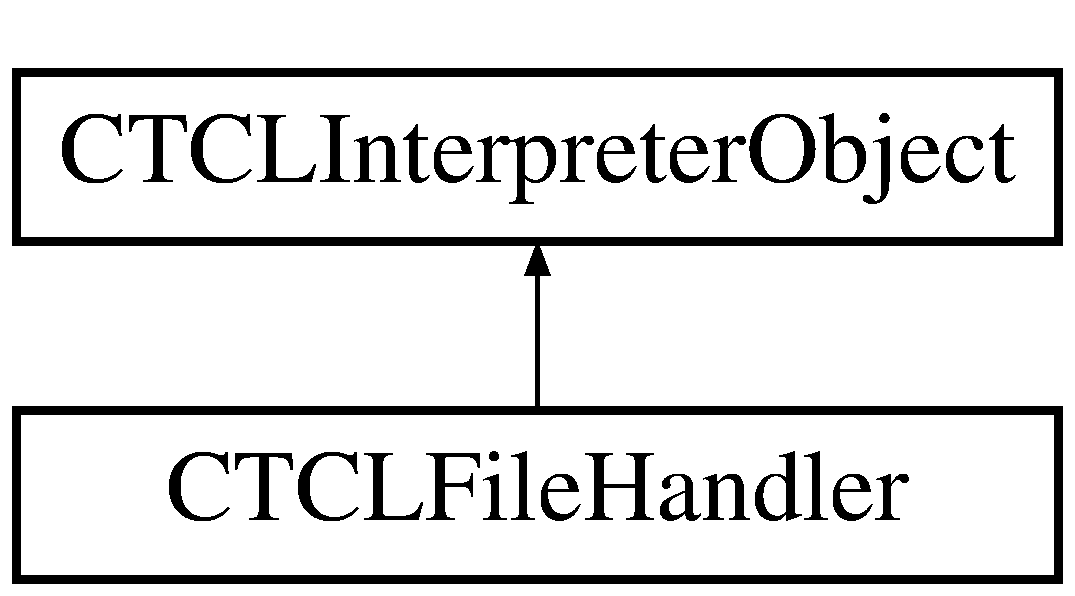
\includegraphics[height=2cm]{classCTCLFileHandler}
\end{center}
\end{figure}
\subsection*{Public Methods}
\begin{CompactItemize}
\item 
{\bf CTCLFile\-Handler} ({\bf CTCLInterpreter\-Object} $\ast$p\-Interp, {\bf UInt\_\-t} am\_\-n\-Fid=STDIN\_\-FILENO)
\item 
{\bf CTCLFile\-Handler} ({\bf CTCLInterpreter\-Object} $\ast$p\-Interp, FILE $\ast$p\-File)
\item 
{\bf CTCLFile\-Handler} ({\bf CTCLInterpreter\-Object} $\ast$p\-Interp, fstream \&r\-File)
\item 
{\bf CTCLFile\-Handler} ({\bf CTCLInterpreter} $\ast$p\-Interp, {\bf UInt\_\-t} am\_\-n\-Fid=STDIN\_\-FILENO)
\item 
{\bf CTCLFile\-Handler} ({\bf CTCLInterpreter} $\ast$p\-Interp, FILE $\ast$p\-File)
\item 
{\bf CTCLFile\-Handler} ({\bf CTCLInterpreter} $\ast$p\-Interp, fstream \&r\-File)
\item 
{\bf $\sim$CTCLFile\-Handler} ()
\item 
{\bf CTCLFile\-Handler} (const CTCLFile\-Handler \&a\-CTCLFile\-Handler)
\item 
CTCLFile\-Handler \& {\bf operator=} (const CTCLFile\-Handler \&a\-CTCLFile\-Handler)
\item 
int {\bf operator==} (const CTCLFile\-Handler \&a\-CTCLFile\-Handler) const
\item 
{\bf UInt\_\-t} {\bf get\-Fid} () const
\item 
void {\bf set\-Fid} ({\bf UInt\_\-t} am\_\-n\-Fid)
\item 
virtual void {\bf operator()} (int mask)=0
\item 
void {\bf Set} (int mask)
\item 
void {\bf Clear} ()
\end{CompactItemize}
\subsection*{Static Public Methods}
\begin{CompactItemize}
\item 
void {\bf Callback\-Relay} (Client\-Data p\-Object, int mask)
\end{CompactItemize}
\subsection*{Private Attributes}
\begin{CompactItemize}
\item 
{\bf UInt\_\-t} {\bf m\_\-n\-Fid}
\end{CompactItemize}


\subsection{Constructor \& Destructor Documentation}
\index{CTCLFileHandler@{CTCLFile\-Handler}!CTCLFileHandler@{CTCLFileHandler}}
\index{CTCLFileHandler@{CTCLFileHandler}!CTCLFileHandler@{CTCLFile\-Handler}}
\subsubsection{\setlength{\rightskip}{0pt plus 5cm}CTCLFile\-Handler::CTCLFile\-Handler ({\bf CTCLInterpreter\-Object} $\ast$ {\em p\-Interp}, {\bf UInt\_\-t} {\em am\_\-n\-Fid} = STDIN\_\-FILENO)\hspace{0.3cm}{\tt  [inline]}}\label{classCTCLFileHandler_a0}




Definition at line 327 of file TCLFile\-Handler.h.

References CTCLInterpreter\-Object::get\-Interpreter(), m\_\-n\-Fid, and UInt\_\-t.\index{CTCLFileHandler@{CTCLFile\-Handler}!CTCLFileHandler@{CTCLFileHandler}}
\index{CTCLFileHandler@{CTCLFileHandler}!CTCLFileHandler@{CTCLFile\-Handler}}
\subsubsection{\setlength{\rightskip}{0pt plus 5cm}CTCLFile\-Handler::CTCLFile\-Handler ({\bf CTCLInterpreter\-Object} $\ast$ {\em p\-Interp}, FILE $\ast$ {\em p\-File})\hspace{0.3cm}{\tt  [inline]}}\label{classCTCLFileHandler_a1}




Definition at line 332 of file TCLFile\-Handler.h.

References CTCLInterpreter\-Object::get\-Interpreter(), and m\_\-n\-Fid.\index{CTCLFileHandler@{CTCLFile\-Handler}!CTCLFileHandler@{CTCLFileHandler}}
\index{CTCLFileHandler@{CTCLFileHandler}!CTCLFileHandler@{CTCLFile\-Handler}}
\subsubsection{\setlength{\rightskip}{0pt plus 5cm}CTCLFile\-Handler::CTCLFile\-Handler ({\bf CTCLInterpreter\-Object} $\ast$ {\em p\-Interp}, fstream \& {\em r\-File})\hspace{0.3cm}{\tt  [inline]}}\label{classCTCLFileHandler_a2}




Definition at line 337 of file TCLFile\-Handler.h.

References m\_\-n\-Fid.\index{CTCLFileHandler@{CTCLFile\-Handler}!CTCLFileHandler@{CTCLFileHandler}}
\index{CTCLFileHandler@{CTCLFileHandler}!CTCLFileHandler@{CTCLFile\-Handler}}
\subsubsection{\setlength{\rightskip}{0pt plus 5cm}CTCLFile\-Handler::CTCLFile\-Handler ({\bf CTCLInterpreter} $\ast$ {\em p\-Interp}, {\bf UInt\_\-t} {\em am\_\-n\-Fid} = STDIN\_\-FILENO)\hspace{0.3cm}{\tt  [inline]}}\label{classCTCLFileHandler_a3}




Definition at line 342 of file TCLFile\-Handler.h.

References m\_\-n\-Fid, and UInt\_\-t.\index{CTCLFileHandler@{CTCLFile\-Handler}!CTCLFileHandler@{CTCLFileHandler}}
\index{CTCLFileHandler@{CTCLFileHandler}!CTCLFileHandler@{CTCLFile\-Handler}}
\subsubsection{\setlength{\rightskip}{0pt plus 5cm}CTCLFile\-Handler::CTCLFile\-Handler ({\bf CTCLInterpreter} $\ast$ {\em p\-Interp}, FILE $\ast$ {\em p\-File})\hspace{0.3cm}{\tt  [inline]}}\label{classCTCLFileHandler_a4}




Definition at line 347 of file TCLFile\-Handler.h.

References m\_\-n\-Fid.\index{CTCLFileHandler@{CTCLFile\-Handler}!CTCLFileHandler@{CTCLFileHandler}}
\index{CTCLFileHandler@{CTCLFileHandler}!CTCLFileHandler@{CTCLFile\-Handler}}
\subsubsection{\setlength{\rightskip}{0pt plus 5cm}CTCLFile\-Handler::CTCLFile\-Handler ({\bf CTCLInterpreter} $\ast$ {\em p\-Interp}, fstream \& {\em r\-File})\hspace{0.3cm}{\tt  [inline]}}\label{classCTCLFileHandler_a5}




Definition at line 352 of file TCLFile\-Handler.h.

References m\_\-n\-Fid.\index{CTCLFileHandler@{CTCLFile\-Handler}!~CTCLFileHandler@{$\sim$CTCLFileHandler}}
\index{~CTCLFileHandler@{$\sim$CTCLFileHandler}!CTCLFileHandler@{CTCLFile\-Handler}}
\subsubsection{\setlength{\rightskip}{0pt plus 5cm}CTCLFile\-Handler::$\sim$CTCLFile\-Handler ()\hspace{0.3cm}{\tt  [inline]}}\label{classCTCLFileHandler_a6}




Definition at line 357 of file TCLFile\-Handler.h.

References Clear().\index{CTCLFileHandler@{CTCLFile\-Handler}!CTCLFileHandler@{CTCLFileHandler}}
\index{CTCLFileHandler@{CTCLFileHandler}!CTCLFileHandler@{CTCLFile\-Handler}}
\subsubsection{\setlength{\rightskip}{0pt plus 5cm}CTCLFile\-Handler::CTCLFile\-Handler (const CTCLFile\-Handler \& {\em a\-CTCLFile\-Handler})\hspace{0.3cm}{\tt  [inline]}}\label{classCTCLFileHandler_a7}




Definition at line 360 of file TCLFile\-Handler.h.

References m\_\-n\-Fid.

\subsection{Member Function Documentation}
\index{CTCLFileHandler@{CTCLFile\-Handler}!CallbackRelay@{CallbackRelay}}
\index{CallbackRelay@{CallbackRelay}!CTCLFileHandler@{CTCLFile\-Handler}}
\subsubsection{\setlength{\rightskip}{0pt plus 5cm}void CTCLFile\-Handler::Callback\-Relay (Client\-Data {\em p\-Object}, int {\em mask})\hspace{0.3cm}{\tt  [static]}}\label{classCTCLFileHandler_d0}




Definition at line 321 of file TCLFile\-Handler.cpp.

Referenced by Set().\index{CTCLFileHandler@{CTCLFile\-Handler}!Clear@{Clear}}
\index{Clear@{Clear}!CTCLFileHandler@{CTCLFile\-Handler}}
\subsubsection{\setlength{\rightskip}{0pt plus 5cm}void CTCLFile\-Handler::Clear ()}\label{classCTCLFileHandler_a14}




Definition at line 372 of file TCLFile\-Handler.cpp.

References m\_\-n\-Fid.

Referenced by $\sim$CTCLFile\-Handler().\index{CTCLFileHandler@{CTCLFile\-Handler}!getFid@{getFid}}
\index{getFid@{getFid}!CTCLFileHandler@{CTCLFile\-Handler}}
\subsubsection{\setlength{\rightskip}{0pt plus 5cm}{\bf UInt\_\-t} CTCLFile\-Handler::get\-Fid () const\hspace{0.3cm}{\tt  [inline]}}\label{classCTCLFileHandler_a10}




Definition at line 388 of file TCLFile\-Handler.h.

References m\_\-n\-Fid, and UInt\_\-t.\index{CTCLFileHandler@{CTCLFile\-Handler}!operator()@{operator()}}
\index{operator()@{operator()}!CTCLFileHandler@{CTCLFile\-Handler}}
\subsubsection{\setlength{\rightskip}{0pt plus 5cm}virtual void CTCLFile\-Handler::operator() (int {\em mask})\hspace{0.3cm}{\tt  [pure virtual]}}\label{classCTCLFileHandler_a12}


\index{CTCLFileHandler@{CTCLFile\-Handler}!operator=@{operator=}}
\index{operator=@{operator=}!CTCLFileHandler@{CTCLFile\-Handler}}
\subsubsection{\setlength{\rightskip}{0pt plus 5cm}CTCLFile\-Handler\& CTCLFile\-Handler::operator= (const CTCLFile\-Handler \& {\em a\-CTCLFile\-Handler})\hspace{0.3cm}{\tt  [inline]}}\label{classCTCLFileHandler_a8}




Definition at line 369 of file TCLFile\-Handler.h.

References m\_\-n\-Fid, and CTCLInterpreter\-Object::operator=().\index{CTCLFileHandler@{CTCLFile\-Handler}!operator==@{operator==}}
\index{operator==@{operator==}!CTCLFileHandler@{CTCLFile\-Handler}}
\subsubsection{\setlength{\rightskip}{0pt plus 5cm}int CTCLFile\-Handler::operator== (const CTCLFile\-Handler \& {\em a\-CTCLFile\-Handler}) const\hspace{0.3cm}{\tt  [inline]}}\label{classCTCLFileHandler_a9}




Definition at line 379 of file TCLFile\-Handler.h.

References m\_\-n\-Fid, and CTCLInterpreter\-Object::operator==().\index{CTCLFileHandler@{CTCLFile\-Handler}!Set@{Set}}
\index{Set@{Set}!CTCLFileHandler@{CTCLFile\-Handler}}
\subsubsection{\setlength{\rightskip}{0pt plus 5cm}void CTCLFile\-Handler::Set (int {\em mask})}\label{classCTCLFileHandler_a13}




Definition at line 348 of file TCLFile\-Handler.cpp.

References Callback\-Relay(), and m\_\-n\-Fid.\index{CTCLFileHandler@{CTCLFile\-Handler}!setFid@{setFid}}
\index{setFid@{setFid}!CTCLFileHandler@{CTCLFile\-Handler}}
\subsubsection{\setlength{\rightskip}{0pt plus 5cm}void CTCLFile\-Handler::set\-Fid ({\bf UInt\_\-t} {\em am\_\-n\-Fid})\hspace{0.3cm}{\tt  [inline]}}\label{classCTCLFileHandler_a11}




Definition at line 395 of file TCLFile\-Handler.h.

References m\_\-n\-Fid, and UInt\_\-t.

\subsection{Member Data Documentation}
\index{CTCLFileHandler@{CTCLFile\-Handler}!m_nFid@{m\_\-nFid}}
\index{m_nFid@{m\_\-nFid}!CTCLFileHandler@{CTCLFile\-Handler}}
\subsubsection{\setlength{\rightskip}{0pt plus 5cm}{\bf UInt\_\-t} CTCLFile\-Handler::m\_\-n\-Fid\hspace{0.3cm}{\tt  [private]}}\label{classCTCLFileHandler_o0}




Definition at line 322 of file TCLFile\-Handler.h.

Referenced by Clear(), CTCLFile\-Handler(), get\-Fid(), operator=(), operator==(), Set(), and set\-Fid().

The documentation for this class was generated from the following files:\begin{CompactItemize}
\item 
{\bf TCLFile\-Handler.h}\item 
{\bf TCLFile\-Handler.cpp}\end{CompactItemize}
